\sffamily\large\justify

\pagenumbering{arabic}

\section{Cinemática directa}

\subsection{Modelado del \emph{youBot Arm}}

\begin{figure}[h!]
    \centering
    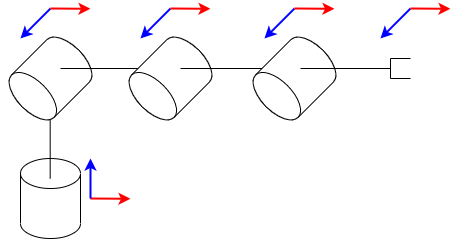
\includegraphics[width=\linewidth]{youBot.png}
    \caption{\sffamily youBot Arm}
    \label{fig:youBotArmModel}
\end{figure}

\subsection{Fórmulas y propiedades}

\begin{equation*}
    ^{n-1}T_n =
    \begin{bmatrix}
        C_{\theta_n} & -S_{\theta_n}C_{\alpha_n} & S_{\theta_n}S_{\alpha_n} & a_nC_{\theta_n} \\
        S_{\theta_n} & C_{\theta_n}C_{\alpha_n} & -C_{\theta_n}S_{\alpha_n} & a_nS_{\theta_n} \\
        0 & S_{\alpha_n} & C_{\alpha_n} & d_n \\
        0 & 0 & 0 & 1
    \end{bmatrix}
\end{equation*}

\begin{equation*}
    \begin{split}
        \sin(\alpha \pm \beta) & = \sin(\alpha)\cos(\beta) \pm \cos(\alpha)\sin(\beta) \\
        \cos(\alpha \pm \beta) & = \cos(\alpha)\cos(\beta) \mp \sin(\alpha)\sin(\beta)
    \end{split}
\end{equation*}

\newpage
\subsection{Tabla de parámetros \emph{Denavit-Hartenberg}}

\begin{table}[h!]
    \centering\sffamily\large

    \begin{tabular}{|c|c|c|c|c|}
        \hline
        & $\alpha$ & $a$ & $d$ & $\theta$ \\
        \hline
        1 & $\frac{\pi}{2}$ & $0$ & $d_1$ & $0$ \\
        \hline
        2 & $0$ & $a_2$ & $0$ & $0$ \\
        \hline
        3 & $0$ & $a_3$ & $0$ & $0$ \\
        \hline
        4 & $0$ & $a_4$ & $0$ & $0$ \\
        \hline
    \end{tabular}

    \caption{\sffamily Tabla de parámetros \emph{Denavit-Hartenberg}}
    \label{tab:tablaDH}
\end{table}

\subsection{Matrices de transformación}

\begin{equation*}
    \tcboxmath[colback=white, colframe=black]{
    ^0T_1 =
    \begin{bmatrix}
        C_1 & 0 & S_1 & 0 \\
        S_1 & 0 & -C_1 & 0 \\
        0 & 0 & 1 & 0 \\
        0 & 0 & 0 & 1
    \end{bmatrix}
    }
    \quad\quad
    ^1T_2 =
    \begin{bmatrix}
        C_2 & -S_2 & 0 & a_2C_2 \\
        S_2 & C_2 & 0 & a_2S_2 \\
        0 & 0 & 1 & 0 \\
        0 & 0 & 0 & 1
    \end{bmatrix}
\end{equation*}

\begin{equation*}
    ^2T_3 =
    \begin{bmatrix}
        C_3 & -S_3 & 0 & a_3C_3 \\
        S_3 & C_3 & 0 & a_3S_3 \\
        0 & 0 & 1 & 0 \\
        0 & 0 & 0 & 1
    \end{bmatrix}
    \quad\quad
    ^3T_4 =
    \begin{bmatrix}
        C_4 & -S_4 & 0 & a_4C_4 \\
        S_4 & C_4 & 0 & a_4S_4 \\
        0 & 0 & 1 & 0 \\
        0 & 0 & 0 & 1
    \end{bmatrix}
\end{equation*}

\begin{equation*}
    ^0T_4 = {^0T_1} \, {^1T_2} \, {^2T_3} \, {^3T_4}
\end{equation*}

\newpage
\subsection{Cinemática directa del \emph{youBot Arm}}

\begin{equation*}
    \tcboxmath[colback=white, colframe=black]{
    ^0T_2 =
    \begin{bmatrix}
        C_1C_2 & -C_1S_2 & S_1 & a_2C_1C_2 \\
        S_1C_2 & -S_1S_2 & -C_1 & a_2S_1C_2 \\
        S_2 & C_2 & 0 & a_2S_2 + d_1 \\
        0 & 0 & 0 & 1
    \end{bmatrix}
    }
\end{equation*}

{\small
\begin{equation*}
    ^0T_3 =
    \begin{bmatrix}
        C_1C_2C_3 - C_1S_2S_3 & -C_1C_2S_3 - C_1S_2C_3 & S_1 & a_3C_1C_2C_3 - a_3C_1S_2S_3 + a_2C_1C_2 \\
        S_1C_2C_3 - S_1S_2S_3 & -S_1C_2S_3 - S_1S_2C_3 & -C_1 & a_3S_1C_2C_3 - a_3S_1S_2S_3 + a_2S_1C_2 \\
        S_2C_3 + C_2S_3 & -S_2S_3 + C_2C_3 & 0 & a_3S_2C_3 + a_3C_2S_3 + a_2S_2 + d_1 \\
        0 & 0 & 0 & 1
    \end{bmatrix}
\end{equation*}
}

\begin{equation*}
    \tcboxmath[colback=white, colframe=black]{
    ^0T_3 =
    \begin{bmatrix}
        C_1C_{23} & -C_1S_{23} & S_1 & a_3C_1C_{23} + a_2C_1C_2 \\
        S_1C_{23} & -S_1S_{23} & -C_1 & a_3S_1C_{23} + a_2S_1C_2 \\
        S_{23} & C_{23} & 0 & a_3S_{23} + a_2S_2 + d_1 \\
        0 & 0 & 0 & 1
    \end{bmatrix}
    }
\end{equation*}

{\scriptsize
\begin{equation*}
    ^0T_4 =
    \begin{bmatrix}
        C_1C_{23}C_4 - C_1S_{23}S_4 & -C_1C_{23}S_4 - C_1S_{23}C_4 & S_1 & a_4C_1C_{23}C_4 - a_4C_1S_{23}S_4 + a_3C_1C_{23} + a_2C_1C_2 \\
        S_1C_{23}C_4 - S_1S_{23}S_4 & -S_1C_{23}S_4 - S_1S_{23}C_4 & -C_1 & a_4S_1C_{23}C_4 - a_4S_1S_{23}S_4 + a_3S_1C_{23} + a_2S_1C_2 \\
        S_{23}C_4 + C_{23}S_4 & -S_{23}S_4 + C_{23}C_4 & 0 & a_4S_{23}C_4 + a_4C_{23}S_4 + a_3S_{23} + a_2S_2 + d_1 \\
        0 & 0 & 0 & 1
    \end{bmatrix}
\end{equation*}
}

\begin{equation*}
    ^0T_4 =
    \begin{bmatrix}
        C_1C_{234} & -C_1S_{234} & S_1 & a_4C_1C_{234} + a_3C_1C_{23} + a_2C_1C_2 \\
        S_1C_{234} & -S_1S_{234} & -C_1 & a_4S_1C_{234} + a_3S_1C_{23} + a_2C_1C_2 \\
        S_{234} & C_{234} & 0 & a_4S_{234} + a_3S_{23} + a_2S_2 + d_1 \\
        0 & 0 & 0 & 1
    \end{bmatrix}
\end{equation*}

\begin{equation*}
    \tcboxmath[colback=white, colframe=black]{
    ^0T_4 =
    \begin{bmatrix}
        C_1C_{234} & -C_1S_{234} & S_1 & C_1 ( a_4C_{234} + a_3C_{23} + a_2C_2 ) \\
        S_1C_{234} & -S_1S_{234} & -C_1 & S_1 ( a_4C_{234} + a_3C_{23} + a_2C_2 ) \\
        S_{234} & C_{234} & 0 & a_4S_{234} + a_3S_{23} + a_2S_2 + d_1 \\
        0 & 0 & 0 & 1
    \end{bmatrix}
    }
\end{equation*}

\newpage
\subsection{Cinemática directa de la plataforma omnidireccional}

\begin{equation*}
    \begin{bmatrix}
        \dot{x} \\
        \dot{y} \\
        \dot{\theta}
    \end{bmatrix} =
    \begin{bmatrix}
        \cos(\theta) & -\sin(\theta) & 0 \\
        \sin(\theta) & \cos(\theta) & 0 \\
        0 & 0 & 1
    \end{bmatrix}
    \begin{bmatrix}
        1 & -1 & -(L+l) \\
        1 & 1 & (L+l) \\
        1 & 1 & -(L+l) \\
        1 & -1 & (L+l)
    \end{bmatrix}^\dagger
    \begin{bmatrix}
        v_1 \\
        v_2 \\
        v_3 \\
        v_4
    \end{bmatrix}
\end{equation*}

\subsection{Cinemática inversa de la plataforma omnidireccional}

\begin{equation*}
    \begin{bmatrix}
        v_1 \\
        v_2 \\
        v_3 \\
        v_4
    \end{bmatrix} =
    \begin{bmatrix}
        1 & -1 & -(L+l) \\
        1 & 1 & (L+l) \\
        1 & 1 & -(L+l) \\
        1 & -1 & (L+l)
    \end{bmatrix}
    \begin{bmatrix}
        \cos(\theta) & -\sin(\theta) & 0 \\
        \sin(\theta) & \cos(\theta) & 0 \\
        0 & 0 & 1
    \end{bmatrix}^\top
    \begin{bmatrix}
        \dot{x} \\
        \dot{y} \\
        \dot{\theta}
    \end{bmatrix}
\end{equation*}

\begin{equation*}
    \begin{bmatrix}
        v_1 \\
        v_2 \\
        v_3 \\
        v_4
    \end{bmatrix} =
    \begin{bmatrix}
        \sqrt{2}\sin(\alpha) & -\sqrt{2}\cos(\alpha) & -(L+l) \\
        \sqrt{2}\cos(\alpha) & \sqrt{2}\sin(\alpha) & (L+l) \\
        \sqrt{2}\cos(\alpha) & \sqrt{2}\sin(\alpha) & -(L+l) \\
        \sqrt{2}\sin(\alpha) & -\sqrt{2}\cos(\alpha) & (L+l)
    \end{bmatrix}
    \begin{bmatrix}
        \dot{x} \\
        \dot{y} \\
        \dot{\theta}
    \end{bmatrix}
\end{equation*}

\begin{equation*}
    \alpha = \theta + \frac{\pi}{4}
\end{equation*}

\newpage
\subsection{Cinemática directa desde el origen hasta el efector final}

\renewcommand{\labelitemi}{$\bullet$}
\begin{itemize}
    \item \textbf{w:} Eje coordenado del origen.
    \item \textbf{p:} Eje coordenado adherido a la plataforma.
    \item \textbf{b:} Eje coordenado de la base del manipulador.
    \item \textbf{e:} Eje coordenado del actuador final.
\end{itemize}

\begin{equation*}
    ^wT_e = {^wT_p} \, {^pT_b} \, {^bT_e}
\end{equation*}

\begin{equation*}
    \tcboxmath[colback=white, colframe=black]{
    ^wT_p =
    \begin{bmatrix}
        \cos(\theta_p) & -\sin(\theta_p) & 0 & x_p \\
        \sin(\theta_p) & \cos(\theta_p) & 0 & y_p \\
        0 & 0 & 1 & 0 \\
        0 & 0 & 0 & 1
    \end{bmatrix}
    }
\end{equation*}

\hspace{0.5cm} Con $x_p$ y $y_p$ como la posición del robot y $\theta_p$ como la
orientación.

\begin{equation*}
    \tcboxmath[colback=white, colframe=black]{
    ^pT_b =
    \begin{bmatrix}
        1 & 0 & 0 & 0.170 \\
        0 & 1 & 0 & 0 \\
        0 & 0 & 1 & 0.060 \\
        0 & 0 & 0 & 1
    \end{bmatrix}
    }
\end{equation*}

\begin{equation*}
    \tcboxmath[colback=white, colframe=black]{
    ^bT_e = {^0T_4}
    }
\end{equation*}

\begin{equation*}
    \tcboxmath[colback=white, colframe=black]{
    ^wT_b =
    \begin{bmatrix}
        \cos(\theta_p) & -\sin(\theta_p) & 0 & 0.170\cos(\theta_p) + x_p \\
        \sin(\theta_p) & \cos(\theta_p) & 0 & 0.170\sin(\theta_p) + y_p \\
        0 & 0 & 1 & 0.060 \\
        0 & 0 & 0 & 1
    \end{bmatrix}
    }
\end{equation*}

\newpage
{\normalsize
\begin{equation*}
    \tcboxmath[colback=white, colframe=black]{
    \begin{split}
        x & = C_\theta C_1( a_4C_{234}+a_3C_{23}+a_2C_2 ) - S_\theta S_1( a_4C_{234}+a_3C_{23}+a_2C_2 ) + 0.170C_\theta + x_p \\
        y & = S_\theta C_1( a_4C_{234}+a_3C_{23}+a_2C_2 ) + C_\theta S_1( a_4C_{234}+a_3C_{23}+a_2C_2 ) + 0.170S_\theta + y_p \\
        z & = a_4S_{234} + a_3S_{23} + a_2S_2 + d_1 + 0.060 \\
    \end{split}
    }
\end{equation*}
}

{\normalsize
\begin{equation*}
    \tcboxmath[colback=white, colframe=black]{
    ^wT_e =
    \begin{bmatrix}
        C_\theta C_1C_{234} - S_\theta S_1C_{234} & -C_\theta C_1S_{234} + S_\theta S_1S_{234} & C_\theta S_1 + S_\theta C_1 & x \\
        S_\theta C_1 C_{234} + C_\theta S_1C_{234} & -S_\theta C_1S_{234} - C_\theta S_1S_{234} & S_\theta S_1 - C_\theta C_1 & y \\
        S_{234} & C_{234} & 0 & z \\
        0 & 0 & 0 & 1
    \end{bmatrix}
    }
\end{equation*}
}

{\normalsize
\begin{equation*}
    \tcboxmath[colback=white, colframe=black]{
    ^wT_e =
    \begin{bmatrix}
        C_{\theta 1}C_{234} & -C_{\theta 1}S_{234} & S_{\theta 1} & C_{\theta 1} ( a_4C_{234} + a_3C_{23} + a_2C_2 ) + 0.170C_\theta + x_p \\
        S_{\theta 1}C_{234} & -S_{\theta 1}S_{234} & -C_{\theta 1} & S_{\theta 1} ( a_4C_{234} + a_3C_{23} + a_2C_2 ) + 0.170S_\theta + y_p \\
        S_{234} & C_{234} & 0 & a_4S_{234} + a_3S_{23} + a_2S_2 + d_1 + 0.060 \\
        0 & 0 & 0 & 1
    \end{bmatrix}
    }
\end{equation*}
}

\subsection{Cinemática diferencial}

\begin{equation*}
    J_v(q) =
    \begin{bmatrix}
        \dfrac{\partial p_1(q)}{\partial q_1} & \dfrac{\partial p_1(q)}{\partial q_2} & \dotsc & \dfrac{\partial p_1(q)}{\partial q_n} \\
        \dfrac{\partial p_2(q)}{\partial q_1} & \dfrac{\partial p_2(q)}{\partial q_2} & \dotsc & \dfrac{\partial p_2(q)}{\partial q_n} \\
        \vdots & \vdots & \ddots & \vdots \\
        \dfrac{\partial p_m(1)}{\partial q_1} & \dfrac{\partial p_m(q)}{\partial q_2} & \dotsc & \dfrac{\partial p_m(q)}{\partial q_n}
    \end{bmatrix}
\end{equation*}

\begin{equation*}
    \begin{split}
        t_x & = C_{\theta 1} ( a_4C_{234} + a_3C_{23} + a_2C_2 ) + 0.170C_\theta + x_p \\
        t_y & = S_{\theta 1} ( a_4C_{234} + a_3C_{23} + a_2C_2 ) + 0.170S_\theta + y_p \\
        t_z & = a_4S_{234} + a_3S_{23} + a_2S_2 + d_1 + 0.060
    \end{split}
\end{equation*}

\newpage
\begin{equation*}
    \begin{split}
        \frac{\partial t_x}{\partial x_p} & = 1 \\
        \frac{\partial t_x}{\partial y_p} & = 0 \\
        \frac{\partial t_x}{\partial \theta_p} & = -S_{\theta 1} ( a_4C_{234}+a_3C_{23}+a_2C_2 ) - 0.170S_\theta \\
        \frac{\partial t_x}{\partial \theta_1} & = -S_{\theta 1} ( a_4C_{234}+a_3C_{23}+a_2C_2 ) \\
        \frac{\partial t_x}{\partial \theta_2} & = -C_{\theta 1} ( a_4S_{234}+a_3S_{23}+a_2S_2 ) \\
        \frac{\partial t_x}{\partial \theta_3} & = -C_{\theta 1} ( a_4S_{234}+a_3S_{23} ) \\
        \frac{\partial t_x}{\partial \theta_4} & = -a_4C_{\theta 1}S_{234}
    \end{split}
\end{equation*}

\begin{equation*}
    \begin{split}
        \frac{\partial t_y}{\partial x_p} & = 0 \\
        \frac{\partial t_y}{\partial y_p} & = 1 \\
        \frac{\partial t_y}{\partial \theta_p} & = C_{\theta 1} ( a_4C_{234} + a_3C_{23} + a_2C_2 ) + 0.170C_\theta \\
        \frac{\partial t_y}{\partial \theta_1} & = C_{\theta 1} ( a_4C_{234} + a_3C_{23} + a_2C_2 )  \\
        \frac{\partial t_y}{\partial \theta_2} & = -S_{\theta 1} ( a_4S_{234} + a_3S_{23} + a_2S_2 ) \\
        \frac{\partial t_y}{\partial \theta_3} & = -S_{\theta 1} ( a_4S_{234} + a_3S_{23} ) \\
        \frac{\partial t_y}{\partial \theta_4} & = -a_4S_{\theta 1}S_{234}
    \end{split}
\end{equation*}

\newpage
\begin{equation*}
    \begin{split}
        \frac{\partial t_z}{\partial x_p} & = 0 \\
        \frac{\partial t_z}{\partial x_p} & = 0 \\
        \frac{\partial t_z}{\partial x_p} & = 0 \\
        \frac{\partial t_z}{\partial \theta_1} & = 0 \\
        \frac{\partial t_z}{\partial \theta_2} & = a_4C_{234} + a_3C_{23} + a_2C_2 \\
        \frac{\partial t_z}{\partial \theta_3} & = a_4C_{234} + a_3C_{23} \\
        \frac{\partial t_z}{\partial \theta_4} & = a_4C_{234}
    \end{split}
\end{equation*}

\begin{equation*}
    J_v =
    \begin{bmatrix}
        \dfrac{\partial t_x}{\partial x_p} & \dfrac{\partial t_x}{\partial y_p} & \dfrac{\partial t_x}{\partial \theta_p} & \dfrac{\partial t_x}{\partial \theta_1} & \dfrac{\partial t_x}{\partial \theta_2} & \dfrac{\partial t_x}{\partial \theta_3} & \dfrac{\partial t_x}{\partial \theta_4} \\
        \dfrac{\partial t_y}{\partial x_p} & \dfrac{\partial t_y}{\partial y_p} & \dfrac{\partial t_y}{\partial \theta_p} & \dfrac{\partial t_y}{\partial \theta_1} & \dfrac{\partial t_y}{\partial \theta_2} & \dfrac{\partial t_y}{\partial \theta_3} & \dfrac{\partial t_y}{\partial \theta_4} \\
        \dfrac{\partial t_z}{\partial x_p} & \dfrac{\partial t_z}{\partial y_p} & \dfrac{\partial t_z}{\partial \theta_p} & \dfrac{\partial t_z}{\partial \theta_1} & \dfrac{\partial t_z}{\partial \theta_2} & \dfrac{\partial t_z}{\partial \theta_3} & \dfrac{\partial t_z}{\partial \theta_4} \\
    \end{bmatrix}
\end{equation*}

